\chapter{Design del sistema}

% ======================================================
%
% 2.1 - ARCHITECTURE
%
% ======================================================
\section{Architettura generale}
Il progetto segue il pattern \emph{Model-View-Controller}, con un package per ogni parte:
La logica fisica è scritta una sola volta, in \texttt{AbstractNBodySimulation}, una classe astratta che offre i metodi \texttt{updateVelocity(b)} e \texttt{updatePosition(b)} sul singolo corpo.
Le sottoclassi decidono solo \emph{come} eseguire le due fasi su tutti i corpi, in sequenza, con dei thread oppure con un executor: è il pattern \emph{Template Method}, mostrato in \cref{fig:gerarchia}.
In questo modo le versioni concorrenti si occupano solo di dividere il lavoro e di sincronizzarsi, e il controller può usarle tutte allo stesso modo.

\begin{figure}[H]
  \centering
  \begin{tikzpicture}[
      box/.style={draw, rounded corners=2pt, fill=gray!8, minimum height=0.8cm,
        inner xsep=6pt, font=\ttfamily\small},
      gen/.style={-{Triangle[open, length=7pt, width=7pt]}}]
    \node[box] (api) {\shortstack{\textit{\small interfaccia}\\NBodySimulation}};
    \node[box, below=0.7cm of api] (abs) {AbstractNBodySimulation};
    \node[box, below=1.1cm of abs] (thr) {ThreadNBodySimulation};
    \node[box, left=0.35cm of thr] (seq) {SequentialNBodySimulation};
    \node[box, right=0.35cm of thr] (exe) {ExecutorNBodySimulation};
    \draw[gen, dashed] (abs) -- (api);
    \draw[gen] (thr) -- (abs);
    \draw[gen] (seq.north) |- ($(abs.south)!0.5!(thr.north)$) -| (abs.south);
    \draw[gen] (exe.north) |- ($(abs.south)!0.5!(thr.north)$) -| (abs.south);
  \end{tikzpicture}
  \caption{Gerarchia delle simulazioni: le sottoclassi implementano \texttt{computeStep()}.}
  \label{fig:gerarchia}
\end{figure}

% ======================================================
%
% 2.2 - SYNCHRONIZATION MONITORS
%
% ======================================================
\section{Monitor di sincronizzazione}
\label{sec:monitor}
Come richiesto dalle specifiche, la coordinazione tra i thread della versione multithread è affidata a un monitor implementato appositamente, \texttt{MonitorBarrier}.
I suoi metodi sono \texttt{synchronized}, l'attesa avviene tramite \texttt{wait()} all'interno di un ciclo \texttt{while} e ogni cambiamento di stato invoca \texttt{notifyAll()}.

% ======================================================
% 2.2.1 - BARRIER
% ======================================================
\subsection{\texttt{MonitorBarrier}: Barriera ciclica}
\label{subsec:barrier}
La barriera sospende i thread che invocano \texttt{await()} finché non sono arrivati tutti: l'ultimo li risveglia e la riporta allo stato iniziale, così da poterla riutilizzare a ogni passo (\emph{cyclic barrier}).
Se un thread viene interrotto o un \texttt{BodyWorker} termina, la barriera si rompe e sblocca tutti, evitando attese infinite.

% ======================================================
%
% 2.3 - MULTITHREADED VERSION
%
% ======================================================
\section{Versione multithread}
\label{sec:design_thread}

% ======================================================
% 2.3.1 - STRUCTURE
% ======================================================
\subsection{Struttura}
I corpi vengono divisi in tanti blocchi quanti sono i core, e a ogni blocco viene assegnato un worker.
I worker sono creati una volta sola, all'inizio, e vengono riutilizzati per tutti i passi.
Il thread che chiama \texttt{step()}, il \emph{master}, li coordina tramite tre barriere:
\begin{itemize}
  \item \texttt{start}, tra master e worker, per far partire il passo;
  \item \texttt{phase}, tra i soli worker, per separare le due fasi;
  \item \texttt{end}, tra master e worker, per chiudere il passo.
\end{itemize}

% ======================================================
% 2.3.2 - BEHAVIOUR
% ======================================================
\subsection{Comportamento}
Un passo si svolge come in \cref{fig:passo}.
Quando il master arriva su \texttt{start}, i worker partono e calcolano le velocità del proprio blocco.
Chi finisce prima aspetta gli altri su \texttt{phase}; poi tutti aggiornano le posizioni e si ritrovano su \texttt{end}.
A quel punto il master aggiorna il tempo virtuale, mentre i worker tornano ad aspettare su \texttt{start} il passo successivo.
A fine simulazione il master chiama \texttt{shutdown()} e i worker terminano.

\begin{figure}[H]
  \centering
  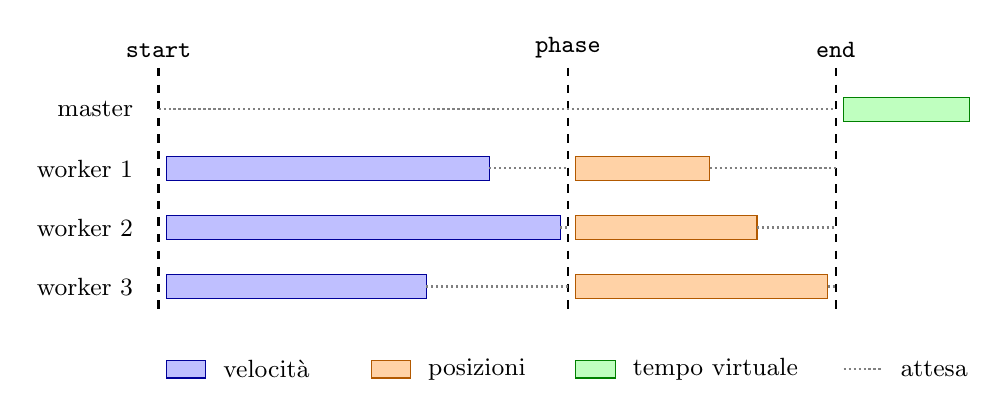
\begin{tikzpicture}[x=1cm, y=0.75cm,
      vel/.style={fill=blue!25, draw=blue!60!black},
      posbar/.style={fill=orange!35, draw=orange!70!black},
      upd/.style={fill=green!25, draw=green!50!black},
      wait/.style={densely dotted, thick, gray}]
    % thread labels
    \foreach \y/\name in {0/master, -1/worker 1, -2/worker 2, -3/worker 3}
      \node[anchor=east, font=\small] at (-0.2, \y) {\name};
    % barriers
    \foreach \x/\name in {0/start, 5.2/phase, 8.6/end}
      \draw[dashed, thick] (\x, 0.7) node[above, font=\ttfamily\small] {\name} -- (\x, -3.5);
    % master
    \draw[wait] (0, 0) -- (8.6, 0);
    \draw[upd] (8.7, -0.2) rectangle (10.3, 0.2);
    % workers: velocities, wait, positions, wait
    \foreach \y/\v/\p in {-1/4.2/7.0, -2/5.1/7.6, -3/3.4/8.5} {
      \draw[vel] (0.1, \y-0.2) rectangle (\v, \y+0.2);
      \draw[wait] (\v, \y) -- (5.2, \y);
      \draw[posbar] (5.3, \y-0.2) rectangle (\p, \y+0.2);
      \draw[wait] (\p, \y) -- (8.6, \y);
    }
    % legend
    \begin{scope}[shift={(0.1, -4.4)}, font=\small]
      \draw[vel] (0, -0.15) rectangle (0.5, 0.15); \node[anchor=west] at (0.6, 0) {velocità};
      \draw[posbar] (2.6, -0.15) rectangle (3.1, 0.15); \node[anchor=west] at (3.2, 0) {posizioni};
      \draw[upd] (5.2, -0.15) rectangle (5.7, 0.15); \node[anchor=west] at (5.8, 0) {tempo virtuale};
      \draw[wait] (8.6, 0) -- (9.1, 0); \node[anchor=west] at (9.2, 0) {attesa};
    \end{scope}
  \end{tikzpicture}
  \caption{Un passo della versione multithread con tre worker.}
  \label{fig:passo}
\end{figure}

La barriera \texttt{phase} garantisce che nessuno aggiorni le posizioni mentre un altro le sta ancora leggendo, mentre \texttt{end} garantisce che il master veda solo stati completi.
Il modello FSP di questo comportamento è descritto nel \cref{chap:fsp}.

% ======================================================
%
% 2.4 - TASK-BASED VERSION
%
% ======================================================
\section{Versione task-based (Executor Framework)}
\label{sec:design_executor}

% ======================================================
% 2.4.1 - STRUCTURE
% ======================================================
\subsection{Struttura}
La versione task-based utilizza un \emph{fixed thread pool}, creato una sola volta e condiviso da tutti i passi.
Anziché dividere i corpi in blocchi, per ogni fase viene creato un task per corpo, e il pool li distribuisce dinamicamente tra i thread (\emph{load balancing}), al costo di $2N$ task per passo.

Non serve una barriera dedicata: il ruolo è svolto da
\begin{center}
  \texttt{CompletableFuture.allOf(...).join()}
\end{center}
che attende il completamento di tutti i task di una fase.

% ======================================================
% 2.4.2 - BEHAVIOUR
% ======================================================
\subsection{Comportamento}
A ogni passo il master sottomette un task \texttt{updateVelocity(b)} per ogni corpo e ne attende il completamento; solo dopo sottomette i task \texttt{updatePosition(b)} e attende di nuovo.
Si ottengono così le stesse garanzie della versione multithread (vedi \cref{sec:design_thread}), con la sincronizzazione delegata all'Executor Framework.

% ======================================================
%
% 2.5 - GUI VERSION
%
% ======================================================
\section{Versione con GUI}
\label{sec:design_gui}

% ======================================================
% 2.5.1 - STRUCTURE
% ======================================================
\subsection{Struttura}
Nella versione con GUI l'utente sceglie quale implementazione eseguire: sequenziale, multithread oppure con Executor.
Il controller lavora sull'interfaccia \texttt{NBodySimulation}, quindi gestisce tutte le versioni allo stesso modo.

Sono coinvolti tre tipi di thread:
\begin{itemize}
  \item l'\emph{Event Dispatch Thread} (EDT) di Swing, che disegna la finestra e gestisce i pulsanti;
  \item il thread della simulazione, che esegue i passi;
  \item gli eventuali thread dell'implementazione scelta, che fanno i calcoli.
\end{itemize}
La simulazione non gira sull'EDT: altrimenti, durante il calcolo, la finestra si bloccherebbe e i pulsanti non risponderebbero.

% ======================================================
% 2.5.2 - SIMULATION CONTROL
% ======================================================
\subsection{Controllo della simulazione}
I pulsanti chiamano i metodi di \texttt{SimulationControl}, che cambiano lo stato del monitor e ritornano subito.
Prima di ogni passo, il thread della simulazione chiama \texttt{awaitNextStep()}: se la simulazione è in pausa aspetta, altrimenti esegue il passo oppure termina.
Gli stati e i comandi che li cambiano sono riportati in \cref{fig:controllo}.

\begin{figure}[H]
  \centering
  \begin{tikzpicture}[
      state/.style={draw, rounded corners=3pt, fill=gray!8, minimum width=2.3cm,
        minimum height=0.8cm, font=\ttfamily\small},
      tr/.style={-{Stealth}, thick},
      lbl/.style={font=\small, fill=white, inner sep=1.5pt}]
    \node[state] (ready) at (0, 0) {READY};
    \node[state] (run) at (4.2, 0) {RUNNING};
    \node[state] (pause) at (8.4, 0) {PAUSED};
    \node[state] (step) at (8.4, -2.6) {STEPPING};
    \node[state, fill=red!10] (stop) at (12.6, -1.3) {STOPPED};
    \draw[tr] (ready) -- node[lbl, above] {start} (run);
    \draw[tr] (ready.south) |- node[lbl, pos=0.75, below] {step} (step);
    \draw[tr] (run) to[bend left=20] node[lbl, above] {pause} (pause);
    \draw[tr] (pause) to[bend left=20] node[lbl, below] {resume} (run);
    \draw[tr] (pause) to[bend left=25] node[lbl, right] {step} (step);
    \draw[tr] (step) to[bend left=25] node[lbl, left] {un passo} (pause);
    \draw[tr] (run) to[loop above, looseness=6] node[lbl, above] {un passo} (run);
    \draw[tr, dashed] ($(stop.west) + (-1.4, 0)$) -- node[lbl, above] {stop} (stop);
  \end{tikzpicture}
  \caption{Stati di \texttt{SimulationControl}. Il comando stop porta in \texttt{STOPPED} da qualsiasi stato.}
  \label{fig:controllo}
\end{figure}

I comandi hanno effetto solo tra un passo e l'altro: una pausa premuta durante un passo lascia finire il passo in corso, così la vista non mostra mai uno stato a metà.
Per disegnare, il thread della simulazione copia le posizioni dei corpi e le passa all'EDT con \texttt{invokeAndWait()}, quindi l'EDT non legge mai i corpi mentre vengono modificati.
